\documentclass[1p]{elsarticle_modified}
%\bibliographystyle{elsarticle-num}

%\usepackage[colorlinks]{hyperref}
%\usepackage{abbrmath_seonhwa} %\Abb, \Ascr, \Acal ,\Abf, \Afrak
\usepackage{amsfonts}
\usepackage{amssymb}
\usepackage{amsmath}
\usepackage{amsthm}
\usepackage{scalefnt}
\usepackage{amsbsy}
\usepackage{kotex}
\usepackage{caption}
\usepackage{subfig}
\usepackage{color}
\usepackage{graphicx}
\usepackage{xcolor} %% white, black, red, green, blue, cyan, magenta, yellow
\usepackage{float}
\usepackage{setspace}
\usepackage{hyperref}

\usepackage{tikz}
\usetikzlibrary{arrows}

\usepackage{multirow}
\usepackage{array} % fixed length table
\usepackage{hhline}

%%%%%%%%%%%%%%%%%%%%%
\makeatletter
\renewcommand*\env@matrix[1][\arraystretch]{%
	\edef\arraystretch{#1}%
	\hskip -\arraycolsep
	\let\@ifnextchar\new@ifnextchar
	\array{*\c@MaxMatrixCols c}}
\makeatother %https://tex.stackexchange.com/questions/14071/how-can-i-increase-the-line-spacing-in-a-matrix
%%%%%%%%%%%%%%%

\usepackage[normalem]{ulem}

\newcommand{\msout}[1]{\ifmmode\text{\sout{\ensuremath{#1}}}\else\sout{#1}\fi}
%SOURCE: \msout is \stkout macro in https://tex.stackexchange.com/questions/20609/strikeout-in-math-mode

\newcommand{\cancel}[1]{
	\ifmmode
	{\color{red}\msout{#1}}
	\else
	{\color{red}\sout{#1}}
	\fi
}

\newcommand{\add}[1]{
	{\color{blue}\uwave{#1}}
}

\newcommand{\replace}[2]{
	\ifmmode
	{\color{red}\msout{#1}}{\color{blue}\uwave{#2}}
	\else
	{\color{red}\sout{#1}}{\color{blue}\uwave{#2}}
	\fi
}

\newcommand{\Sol}{\mathcal{S}} %segment
\newcommand{\D}{D} %diagram
\newcommand{\A}{\mathcal{A}} %arc


%%%%%%%%%%%%%%%%%%%%%%%%%%%%%5 test

\def\sl{\operatorname{\textup{SL}}(2,\Cbb)}
\def\psl{\operatorname{\textup{PSL}}(2,\Cbb)}
\def\quan{\mkern 1mu \triangleright \mkern 1mu}

\theoremstyle{definition}
\newtheorem{thm}{Theorem}[section]
\newtheorem{prop}[thm]{Proposition}
\newtheorem{lem}[thm]{Lemma}
\newtheorem{ques}[thm]{Question}
\newtheorem{cor}[thm]{Corollary}
\newtheorem{defn}[thm]{Definition}
\newtheorem{exam}[thm]{Example}
\newtheorem{rmk}[thm]{Remark}
\newtheorem{alg}[thm]{Algorithm}

\newcommand{\I}{\sqrt{-1}}
\begin{document}

%\begin{frontmatter}
%
%\title{Boundary parabolic representations of knots up to 8 crossings}
%
%%% Group authors per affiliation:
%\author{Yunhi Cho} 
%\address{Department of Mathematics, University of Seoul, Seoul, Korea}
%\ead{yhcho@uos.ac.kr}
%
%
%\author{Seonhwa Kim} %\fnref{s_kim}}
%\address{Center for Geometry and Physics, Institute for Basic Science, Pohang, 37673, Korea}
%\ead{ryeona17@ibs.re.kr}
%
%\author{Hyuk Kim}
%\address{Department of Mathematical Sciences, Seoul National University, Seoul 08826, Korea}
%\ead{hyukkim@snu.ac.kr}
%
%\author{Seokbeom Yoon}
%\address{Department of Mathematical Sciences, Seoul National University, Seoul, 08826,  Korea}
%\ead{sbyoon15@snu.ac.kr}
%
%\begin{abstract}
%We find all boundary parabolic representation of knots up to 8 crossings.
%
%\end{abstract}
%\begin{keyword}
%    \MSC[2010] 57M25 
%\end{keyword}
%
%\end{frontmatter}

%\linenumbers
%\tableofcontents
%
\newcommand\colored[1]{\textcolor{white}{\rule[-0.35ex]{0.8em}{1.4ex}}\kern-0.8em\color{red} #1}%
%\newcommand\colored[1]{\textcolor{white}{ #1}\kern-2.17ex	\textcolor{white}{ #1}\kern-1.81ex	\textcolor{white}{ #1}\kern-2.15ex\color{red}#1	}

{\Large $\underline{12a_{0856}~(K12a_{0856})}$}

\setlength{\tabcolsep}{10pt}
\renewcommand{\arraystretch}{1.6}
\vspace{1cm}\begin{tabular}{m{100pt}>{\centering\arraybackslash}m{274pt}}
\multirow{5}{120pt}{
	\centering
	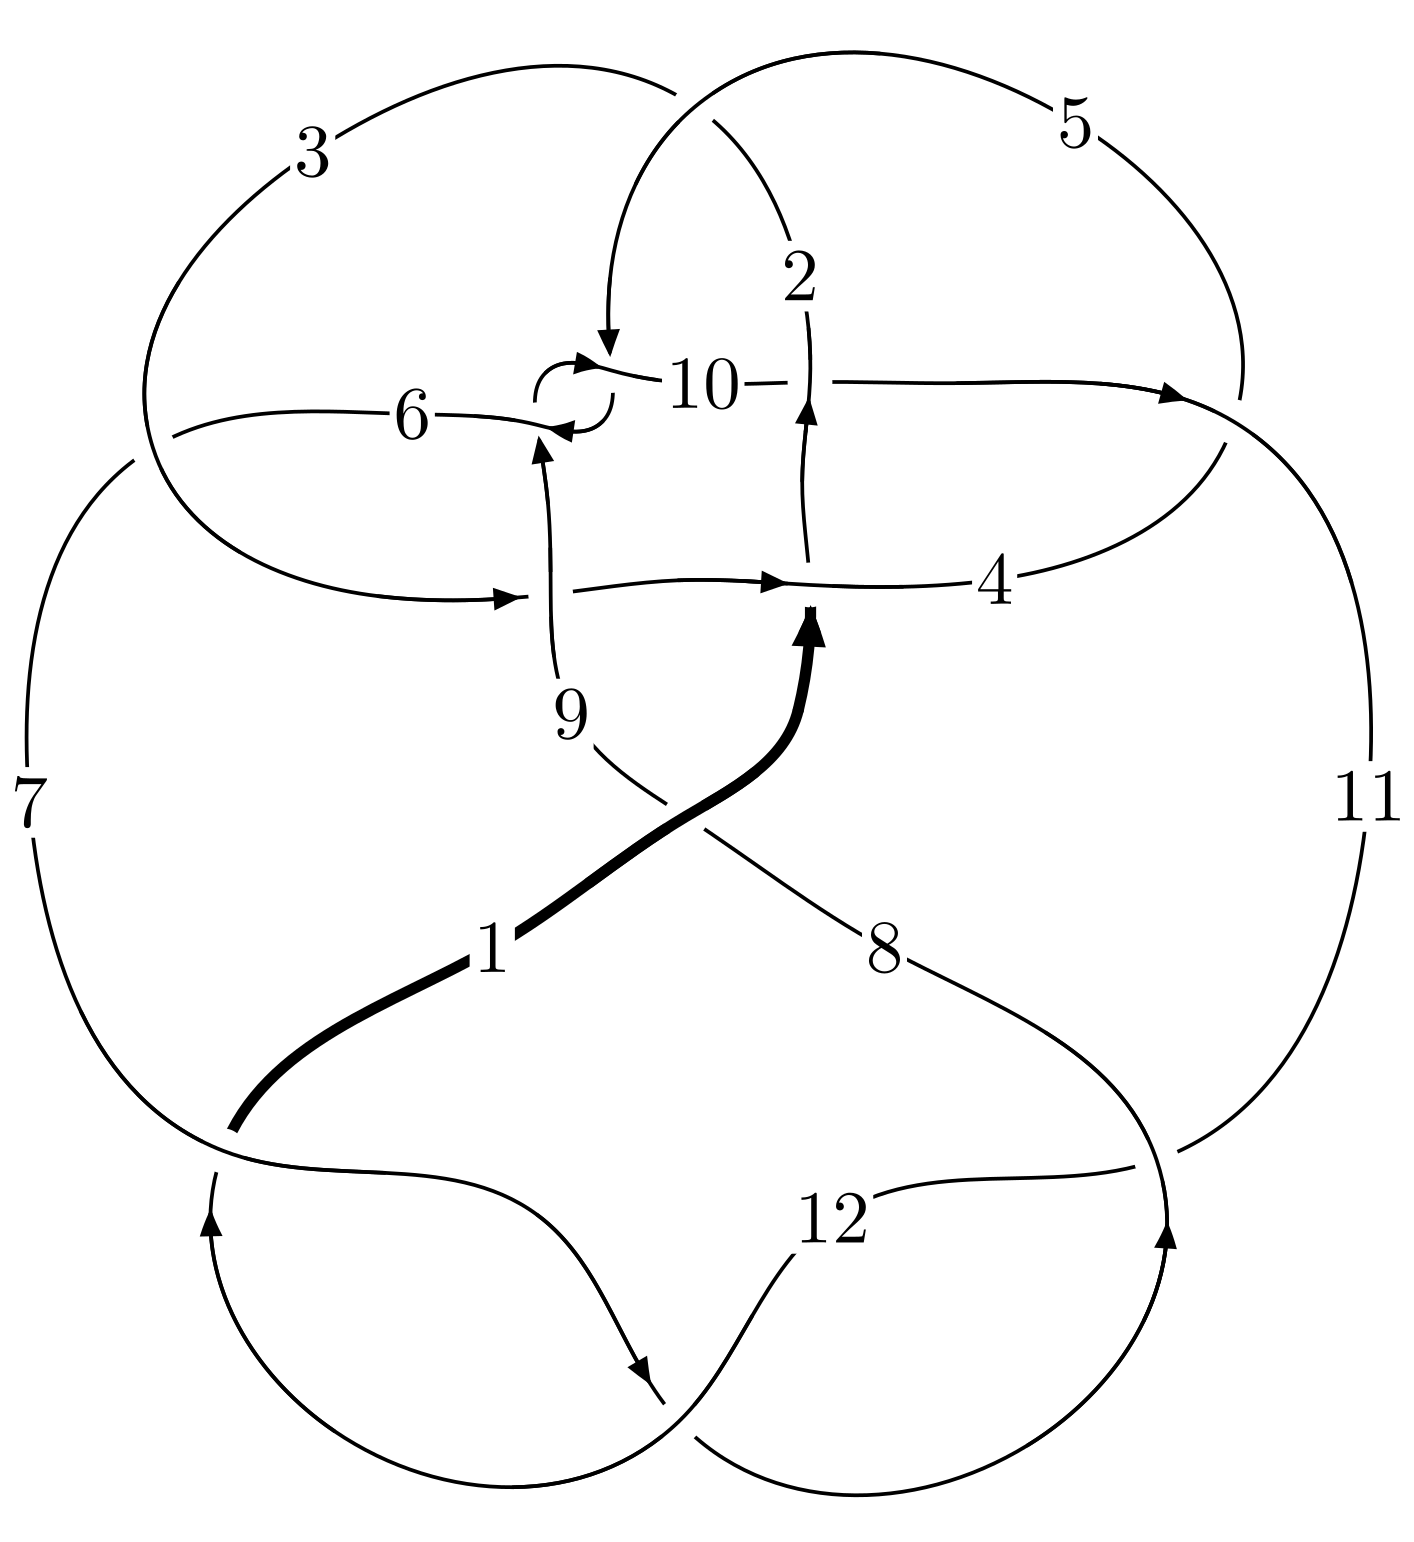
\includegraphics[width=112pt]{../../../GIT/diagram.site/Diagrams/png/1657_12a_0856.png}\\
\ \ \ A knot diagram\footnotemark}&
\allowdisplaybreaks
\textbf{Linearized knot diagam} \\
\cline{2-2}
 &
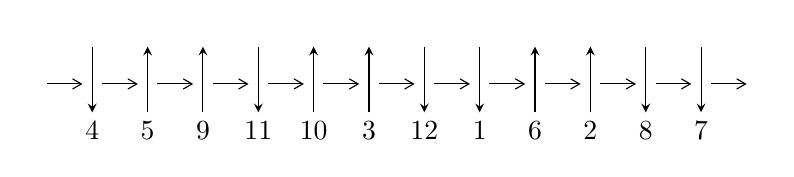
\begin{tikzpicture}[x=20pt, y=17pt]
	% nodes
	\node (C0) at (0, 0) {};
	\node (C1) at (1, 0) {};
	\node (C1U) at (1, +1) {};
	\node (C1D) at (1, -1) {4};

	\node (C2) at (2, 0) {};
	\node (C2U) at (2, +1) {};
	\node (C2D) at (2, -1) {5};

	\node (C3) at (3, 0) {};
	\node (C3U) at (3, +1) {};
	\node (C3D) at (3, -1) {9};

	\node (C4) at (4, 0) {};
	\node (C4U) at (4, +1) {};
	\node (C4D) at (4, -1) {11};

	\node (C5) at (5, 0) {};
	\node (C5U) at (5, +1) {};
	\node (C5D) at (5, -1) {10};

	\node (C6) at (6, 0) {};
	\node (C6U) at (6, +1) {};
	\node (C6D) at (6, -1) {3};

	\node (C7) at (7, 0) {};
	\node (C7U) at (7, +1) {};
	\node (C7D) at (7, -1) {12};

	\node (C8) at (8, 0) {};
	\node (C8U) at (8, +1) {};
	\node (C8D) at (8, -1) {1};

	\node (C9) at (9, 0) {};
	\node (C9U) at (9, +1) {};
	\node (C9D) at (9, -1) {6};

	\node (C10) at (10, 0) {};
	\node (C10U) at (10, +1) {};
	\node (C10D) at (10, -1) {2};

	\node (C11) at (11, 0) {};
	\node (C11U) at (11, +1) {};
	\node (C11D) at (11, -1) {8};

	\node (C12) at (12, 0) {};
	\node (C12U) at (12, +1) {};
	\node (C12D) at (12, -1) {7};
	\node (C13) at (13, 0) {};

	% arrows
	\draw[->,>={angle 60}]
	(C0) edge (C1) (C1) edge (C2) (C2) edge (C3) (C3) edge (C4) (C4) edge (C5) (C5) edge (C6) (C6) edge (C7) (C7) edge (C8) (C8) edge (C9) (C9) edge (C10) (C10) edge (C11) (C11) edge (C12) (C12) edge (C13) ;	\draw[->,>=stealth]
	(C1U) edge (C1D) (C2D) edge (C2U) (C3D) edge (C3U) (C4U) edge (C4D) (C5D) edge (C5U) (C6D) edge (C6U) (C7U) edge (C7D) (C8U) edge (C8D) (C9D) edge (C9U) (C10D) edge (C10U) (C11U) edge (C11D) (C12U) edge (C12D) ;
	\end{tikzpicture} \\
\hhline{~~} \\& 
\textbf{Solving Sequence} \\ \cline{2-2} 
 &
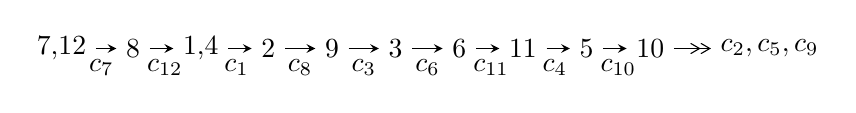
\begin{tikzpicture}[x=23pt, y=7pt]
	% node
	\node (A0) at (-1/8, 0) {7,12};
	\node (A1) at (1, 0) {8};
	\node (A2) at (33/16, 0) {1,4};
	\node (A3) at (25/8, 0) {2};
	\node (A4) at (33/8, 0) {9};
	\node (A5) at (41/8, 0) {3};
	\node (A6) at (49/8, 0) {6};
	\node (A7) at (57/8, 0) {11};
	\node (A8) at (65/8, 0) {5};
	\node (A9) at (73/8, 0) {10};
	\node (C1) at (1/2, -1) {$c_{7}$};
	\node (C2) at (3/2, -1) {$c_{12}$};
	\node (C3) at (21/8, -1) {$c_{1}$};
	\node (C4) at (29/8, -1) {$c_{8}$};
	\node (C5) at (37/8, -1) {$c_{3}$};
	\node (C6) at (45/8, -1) {$c_{6}$};
	\node (C7) at (53/8, -1) {$c_{11}$};
	\node (C8) at (61/8, -1) {$c_{4}$};
	\node (C9) at (69/8, -1) {$c_{10}$};
	\node (A10) at (11, 0) {$c_{2},c_{5},c_{9}$};

	% edge
	\draw[->,>=stealth]	
	(A0) edge (A1) (A1) edge (A2) (A2) edge (A3) (A3) edge (A4) (A4) edge (A5) (A5) edge (A6) (A6) edge (A7) (A7) edge (A8) (A8) edge (A9) ;
	\draw[->>,>={angle 60}]	
	(A9) edge (A10);
\end{tikzpicture} \\ 

\end{tabular} \\

\footnotetext{
The image of knot diagram is generated by the software ``\textbf{Draw programme}" developed by Andrew Bartholomew(\url{http://www.layer8.co.uk/maths/draw/index.htm\#Running-draw}), where we modified some parts for our purpose(\url{https://github.com/CATsTAILs/LinksPainter}).
}\phantom \\ \newline 
\centering \textbf{Ideals for irreducible components\footnotemark of $X_{\text{par}}$} 
 
\begin{align*}
I^u_{1}&=\langle 
7.12526\times10^{207} u^{143}-1.12084\times10^{208} u^{142}+\cdots+7.50129\times10^{207} b-1.99096\times10^{208},\\
\phantom{I^u_{1}}&\phantom{= \langle  }1.56461\times10^{207} u^{143}+2.57970\times10^{208} u^{142}+\cdots+4.87584\times10^{208} a+1.63063\times10^{210},\\
\phantom{I^u_{1}}&\phantom{= \langle  }u^{144}-2 u^{143}+\cdots-50 u+13\rangle \\
I^u_{2}&=\langle 
-8 u^{27}+9 u^{26}+\cdots+2 b-5,\;- u^{27}+5 u^{26}+\cdots+a-4,\;u^{28}- u^{27}+\cdots-9 u^2+1\rangle \\
\\
\end{align*}
\raggedright * 2 irreducible components of $\dim_{\mathbb{C}}=0$, with total 172 representations.\\
\footnotetext{All coefficients of polynomials are rational numbers. But the coefficients are sometimes approximated in decimal forms when there is not enough margin.}
\newpage
\renewcommand{\arraystretch}{1}
\centering \section*{I. $I^u_{1}= \langle 7.13\times10^{207} u^{143}-1.12\times10^{208} u^{142}+\cdots+7.50\times10^{207} b-1.99\times10^{208},\;1.56\times10^{207} u^{143}+2.58\times10^{208} u^{142}+\cdots+4.88\times10^{208} a+1.63\times10^{210},\;u^{144}-2 u^{143}+\cdots-50 u+13 \rangle$}
\flushleft \textbf{(i) Arc colorings}\\
\begin{tabular}{m{7pt} m{180pt} m{7pt} m{180pt} }
\flushright $a_{7}=$&$\begin{pmatrix}1\\0\end{pmatrix}$ \\
\flushright $a_{12}=$&$\begin{pmatrix}0\\u\end{pmatrix}$ \\
\flushright $a_{8}=$&$\begin{pmatrix}1\\u^2\end{pmatrix}$ \\
\flushright $a_{1}=$&$\begin{pmatrix}- u\\u\end{pmatrix}$ \\
\flushright $a_{4}=$&$\begin{pmatrix}-0.0320891 u^{143}-0.529079 u^{142}+\cdots+51.8978 u-33.4430\\-0.949871 u^{143}+1.49419 u^{142}+\cdots-13.0610 u+2.65415\end{pmatrix}$ \\
\flushright $a_{2}=$&$\begin{pmatrix}2.41193 u^{143}-2.44986 u^{142}+\cdots-13.7788 u+6.73154\\-1.24040 u^{143}-0.492406 u^{142}+\cdots+58.6702 u-20.3479\end{pmatrix}$ \\
\flushright $a_{9}=$&$\begin{pmatrix}- u^4- u^2+1\\u^4+2 u^2\end{pmatrix}$ \\
\flushright $a_{3}=$&$\begin{pmatrix}-1.94179 u^{143}+1.00024 u^{142}+\cdots+90.3581 u-53.3307\\-0.242149 u^{143}+2.97935 u^{142}+\cdots-70.3801 u+16.2721\end{pmatrix}$ \\
\flushright $a_{6}=$&$\begin{pmatrix}0.318037 u^{143}-2.37361 u^{142}+\cdots+16.6646 u+5.50682\\0.163273 u^{143}+1.25262 u^{142}+\cdots-39.6022 u+9.52014\end{pmatrix}$ \\
\flushright $a_{11}=$&$\begin{pmatrix}u\\u^3+u\end{pmatrix}$ \\
\flushright $a_{5}=$&$\begin{pmatrix}-1.61419 u^{143}-1.49529 u^{142}+\cdots+136.644 u-64.4507\\-0.655868 u^{143}+5.47078 u^{142}+\cdots-114.268 u+25.3417\end{pmatrix}$ \\
\flushright $a_{10}=$&$\begin{pmatrix}-5.68102 u^{143}+12.2495 u^{142}+\cdots-130.198 u+33.6185\\3.80659 u^{143}-5.90248 u^{142}+\cdots+25.9029 u-3.68074\end{pmatrix}$\\&\end{tabular}
\flushleft \textbf{(ii) Obstruction class $= -1$}\\~\\
\flushleft \textbf{(iii) Cusp Shapes $= -2.07962 u^{143}+1.78992 u^{142}+\cdots+20.9985 u-23.7397$}\\~\\
\newpage\renewcommand{\arraystretch}{1}
\flushleft \textbf{(iv) u-Polynomials at the component}\newline \\
\begin{tabular}{m{50pt}|m{274pt}}
Crossings & \hspace{64pt}u-Polynomials at each crossing \\
\hline $$\begin{aligned}c_{1}\end{aligned}$$&$\begin{aligned}
&u^{144}+12 u^{143}+\cdots+667809 u+245123
\end{aligned}$\\
\hline $$\begin{aligned}c_{2}\end{aligned}$$&$\begin{aligned}
&u^{144}-6 u^{143}+\cdots+381 u+17
\end{aligned}$\\
\hline $$\begin{aligned}c_{3}\end{aligned}$$&$\begin{aligned}
&u^{144}- u^{143}+\cdots-3086919 u+6171839
\end{aligned}$\\
\hline $$\begin{aligned}c_{4}\end{aligned}$$&$\begin{aligned}
&u^{144}- u^{143}+\cdots+11 u+73
\end{aligned}$\\
\hline $$\begin{aligned}c_{5},c_{9}\end{aligned}$$&$\begin{aligned}
&u^{144}-4 u^{143}+\cdots-73 u^2+1
\end{aligned}$\\
\hline $$\begin{aligned}c_{6}\end{aligned}$$&$\begin{aligned}
&u^{144}+3 u^{143}+\cdots+10871 u+1351
\end{aligned}$\\
\hline $$\begin{aligned}c_{7},c_{11},c_{12}\end{aligned}$$&$\begin{aligned}
&u^{144}+2 u^{143}+\cdots+50 u+13
\end{aligned}$\\
\hline $$\begin{aligned}c_{8}\end{aligned}$$&$\begin{aligned}
&u^{144}-2 u^{143}+\cdots+1264438 u+100009
\end{aligned}$\\
\hline $$\begin{aligned}c_{10}\end{aligned}$$&$\begin{aligned}
&u^{144}-8 u^{143}+\cdots-325788 u+55651
\end{aligned}$\\
\hline
\end{tabular}\\~\\
\newpage\renewcommand{\arraystretch}{1}
\flushleft \textbf{(v) Riley Polynomials at the component}\newline \\
\begin{tabular}{m{50pt}|m{274pt}}
Crossings & \hspace{64pt}Riley Polynomials at each crossing \\
\hline $$\begin{aligned}c_{1}\end{aligned}$$&$\begin{aligned}
&y^{144}-20 y^{143}+\cdots+504300454111 y+60085285129
\end{aligned}$\\
\hline $$\begin{aligned}c_{2}\end{aligned}$$&$\begin{aligned}
&y^{144}+18 y^{143}+\cdots+23411 y+289
\end{aligned}$\\
\hline $$\begin{aligned}c_{3}\end{aligned}$$&$\begin{aligned}
&y^{144}+35 y^{143}+\cdots+1367319658441467 y+38091596641921
\end{aligned}$\\
\hline $$\begin{aligned}c_{4}\end{aligned}$$&$\begin{aligned}
&y^{144}+21 y^{143}+\cdots+762145 y+5329
\end{aligned}$\\
\hline $$\begin{aligned}c_{5},c_{9}\end{aligned}$$&$\begin{aligned}
&y^{144}+110 y^{143}+\cdots-146 y+1
\end{aligned}$\\
\hline $$\begin{aligned}c_{6}\end{aligned}$$&$\begin{aligned}
&y^{144}+21 y^{143}+\cdots+108316509 y+1825201
\end{aligned}$\\
\hline $$\begin{aligned}c_{7},c_{11},c_{12}\end{aligned}$$&$\begin{aligned}
&y^{144}+130 y^{143}+\cdots-3852 y+169
\end{aligned}$\\
\hline $$\begin{aligned}c_{8}\end{aligned}$$&$\begin{aligned}
&y^{144}-16 y^{143}+\cdots+335701233910 y+10001800081
\end{aligned}$\\
\hline $$\begin{aligned}c_{10}\end{aligned}$$&$\begin{aligned}
&y^{144}+32 y^{143}+\cdots+173978927610 y+3097033801
\end{aligned}$\\
\hline
\end{tabular}\\~\\
\newpage\flushleft \textbf{(vi) Complex Volumes and Cusp Shapes}
$$\begin{array}{c|c|c}  
\text{Solutions to }I^u_{1}& \I (\text{vol} + \sqrt{-1}CS) & \text{Cusp shape}\\
 \hline 
\begin{aligned}
u &= -0.484439 + 0.833652 I \\
a &= \phantom{-}0.92352 - 1.31726 I \\
b &= -0.944270 + 0.061747 I\end{aligned}
 & \phantom{-}0.71833 - 4.95715 I & \phantom{-0.000000 } 0 \\ \hline\begin{aligned}
u &= -0.484439 - 0.833652 I \\
a &= \phantom{-}0.92352 + 1.31726 I \\
b &= -0.944270 - 0.061747 I\end{aligned}
 & \phantom{-}0.71833 + 4.95715 I & \phantom{-0.000000 } 0 \\ \hline\begin{aligned}
u &= -0.205291 + 1.015960 I \\
a &= -1.12377 + 1.31874 I \\
b &= \phantom{-}0.820159 - 0.200524 I\end{aligned}
 & -0.427059 - 0.972579 I & \phantom{-0.000000 } 0 \\ \hline\begin{aligned}
u &= -0.205291 - 1.015960 I \\
a &= -1.12377 - 1.31874 I \\
b &= \phantom{-}0.820159 + 0.200524 I\end{aligned}
 & -0.427059 + 0.972579 I & \phantom{-0.000000 } 0 \\ \hline\begin{aligned}
u &= \phantom{-}0.476464 + 0.834498 I \\
a &= -1.07044 - 1.42369 I \\
b &= \phantom{-}1.023520 - 0.118162 I\end{aligned}
 & -4.27831 + 10.71680 I & \phantom{-0.000000 } 0 \\ \hline\begin{aligned}
u &= \phantom{-}0.476464 - 0.834498 I \\
a &= -1.07044 + 1.42369 I \\
b &= \phantom{-}1.023520 + 0.118162 I\end{aligned}
 & -4.27831 - 10.71680 I & \phantom{-0.000000 } 0 \\ \hline\begin{aligned}
u &= -0.046308 + 0.940124 I \\
a &= \phantom{-}0.66778 + 2.13397 I \\
b &= -0.012832 - 0.619127 I\end{aligned}
 & -4.39221 + 2.01851 I & \phantom{-0.000000 } 0 \\ \hline\begin{aligned}
u &= -0.046308 - 0.940124 I \\
a &= \phantom{-}0.66778 - 2.13397 I \\
b &= -0.012832 + 0.619127 I\end{aligned}
 & -4.39221 - 2.01851 I & \phantom{-0.000000 } 0 \\ \hline\begin{aligned}
u &= -0.428510 + 0.976666 I \\
a &= -0.870858 + 0.361395 I \\
b &= \phantom{-}0.481560 + 0.463855 I\end{aligned}
 & -0.93362 - 2.08054 I & \phantom{-0.000000 } 0 \\ \hline\begin{aligned}
u &= -0.428510 - 0.976666 I \\
a &= -0.870858 - 0.361395 I \\
b &= \phantom{-}0.481560 - 0.463855 I\end{aligned}
 & -0.93362 + 2.08054 I & \phantom{-0.000000 } 0\\
 \hline 
 \end{array}$$\newpage$$\begin{array}{c|c|c}  
\text{Solutions to }I^u_{1}& \I (\text{vol} + \sqrt{-1}CS) & \text{Cusp shape}\\
 \hline 
\begin{aligned}
u &= -0.302451 + 1.045920 I \\
a &= -0.13758 - 1.92205 I \\
b &= \phantom{-}0.048646 + 0.983005 I\end{aligned}
 & -4.65830 - 2.58703 I & \phantom{-0.000000 } 0 \\ \hline\begin{aligned}
u &= -0.302451 - 1.045920 I \\
a &= -0.13758 + 1.92205 I \\
b &= \phantom{-}0.048646 - 0.983005 I\end{aligned}
 & -4.65830 + 2.58703 I & \phantom{-0.000000 } 0 \\ \hline\begin{aligned}
u &= \phantom{-}0.835501 + 0.351858 I \\
a &= -0.336993 - 0.612412 I \\
b &= \phantom{-}1.64331 + 0.25059 I\end{aligned}
 & -4.67776 - 2.13375 I & \phantom{-0.000000 } 0 \\ \hline\begin{aligned}
u &= \phantom{-}0.835501 - 0.351858 I \\
a &= -0.336993 + 0.612412 I \\
b &= \phantom{-}1.64331 - 0.25059 I\end{aligned}
 & -4.67776 + 2.13375 I & \phantom{-0.000000 } 0 \\ \hline\begin{aligned}
u &= -0.424743 + 1.031960 I \\
a &= -0.30032 - 1.46736 I \\
b &= -0.309462 + 0.700857 I\end{aligned}
 & -5.06551 + 9.60123 I & \phantom{-0.000000 } 0 \\ \hline\begin{aligned}
u &= -0.424743 - 1.031960 I \\
a &= -0.30032 + 1.46736 I \\
b &= -0.309462 - 0.700857 I\end{aligned}
 & -5.06551 - 9.60123 I & \phantom{-0.000000 } 0 \\ \hline\begin{aligned}
u &= \phantom{-}0.532696 + 0.704877 I \\
a &= \phantom{-}0.123811 + 0.332686 I \\
b &= -0.270020 + 0.240025 I\end{aligned}
 & \phantom{-}0.32838 - 1.44483 I & \phantom{-0.000000 } 0 \\ \hline\begin{aligned}
u &= \phantom{-}0.532696 - 0.704877 I \\
a &= \phantom{-}0.123811 - 0.332686 I \\
b &= -0.270020 - 0.240025 I\end{aligned}
 & \phantom{-}0.32838 + 1.44483 I & \phantom{-0.000000 } 0 \\ \hline\begin{aligned}
u &= \phantom{-}0.402671 + 1.068910 I \\
a &= -0.02101 - 1.49837 I \\
b &= \phantom{-}0.381190 + 0.819710 I\end{aligned}
 & -0.25419 - 3.86423 I & \phantom{-0.000000 } 0 \\ \hline\begin{aligned}
u &= \phantom{-}0.402671 - 1.068910 I \\
a &= -0.02101 + 1.49837 I \\
b &= \phantom{-}0.381190 - 0.819710 I\end{aligned}
 & -0.25419 + 3.86423 I & \phantom{-0.000000 } 0\\
 \hline 
 \end{array}$$\newpage$$\begin{array}{c|c|c}  
\text{Solutions to }I^u_{1}& \I (\text{vol} + \sqrt{-1}CS) & \text{Cusp shape}\\
 \hline 
\begin{aligned}
u &= -0.838389 + 0.146060 I \\
a &= \phantom{-}0.019114 + 0.250127 I \\
b &= -1.012750 - 0.457845 I\end{aligned}
 & -7.80704 - 5.07775 I & \phantom{-0.000000 } 0 \\ \hline\begin{aligned}
u &= -0.838389 - 0.146060 I \\
a &= \phantom{-}0.019114 - 0.250127 I \\
b &= -1.012750 + 0.457845 I\end{aligned}
 & -7.80704 + 5.07775 I & \phantom{-0.000000 } 0 \\ \hline\begin{aligned}
u &= -0.802549 + 0.276471 I \\
a &= \phantom{-}0.056196 - 0.221665 I \\
b &= -1.70328 + 0.58339 I\end{aligned}
 & -1.07174 + 9.49563 I & \phantom{-0.000000 } 0 \\ \hline\begin{aligned}
u &= -0.802549 - 0.276471 I \\
a &= \phantom{-}0.056196 + 0.221665 I \\
b &= -1.70328 - 0.58339 I\end{aligned}
 & -1.07174 - 9.49563 I & \phantom{-0.000000 } 0 \\ \hline\begin{aligned}
u &= \phantom{-}0.801348 + 0.276890 I \\
a &= \phantom{-}0.084525 - 0.187889 I \\
b &= \phantom{-}1.85520 + 0.69466 I\end{aligned}
 & -6.0713 - 15.2379 I & \phantom{-0.000000 } 0 \\ \hline\begin{aligned}
u &= \phantom{-}0.801348 - 0.276890 I \\
a &= \phantom{-}0.084525 + 0.187889 I \\
b &= \phantom{-}1.85520 - 0.69466 I\end{aligned}
 & -6.0713 + 15.2379 I & \phantom{-0.000000 } 0 \\ \hline\begin{aligned}
u &= -0.817069 + 0.225836 I \\
a &= \phantom{-}0.232580 - 0.084623 I \\
b &= \phantom{-}0.954296 - 0.841047 I\end{aligned}
 & -3.23396 + 6.58116 I & \phantom{-0.000000 } 0 \\ \hline\begin{aligned}
u &= -0.817069 - 0.225836 I \\
a &= \phantom{-}0.232580 + 0.084623 I \\
b &= \phantom{-}0.954296 + 0.841047 I\end{aligned}
 & -3.23396 - 6.58116 I & \phantom{-0.000000 } 0 \\ \hline\begin{aligned}
u &= \phantom{-}0.770010 + 0.306600 I \\
a &= -0.225784 + 0.058170 I \\
b &= -0.881701 - 0.263466 I\end{aligned}
 & -1.02699 - 2.97737 I & \phantom{-0.000000 } 0 \\ \hline\begin{aligned}
u &= \phantom{-}0.770010 - 0.306600 I \\
a &= -0.225784 - 0.058170 I \\
b &= -0.881701 + 0.263466 I\end{aligned}
 & -1.02699 + 2.97737 I & \phantom{-0.000000 } 0\\
 \hline 
 \end{array}$$\newpage$$\begin{array}{c|c|c}  
\text{Solutions to }I^u_{1}& \I (\text{vol} + \sqrt{-1}CS) & \text{Cusp shape}\\
 \hline 
\begin{aligned}
u &= \phantom{-}0.324296 + 1.128410 I \\
a &= \phantom{-}1.63144 + 0.88501 I \\
b &= -1.38997 + 0.38453 I\end{aligned}
 & -3.37182 + 0.96266 I & \phantom{-0.000000 } 0 \\ \hline\begin{aligned}
u &= \phantom{-}0.324296 - 1.128410 I \\
a &= \phantom{-}1.63144 - 0.88501 I \\
b &= -1.38997 - 0.38453 I\end{aligned}
 & -3.37182 - 0.96266 I & \phantom{-0.000000 } 0 \\ \hline\begin{aligned}
u &= \phantom{-}0.508667 + 0.642306 I \\
a &= -0.45841 - 1.42683 I \\
b &= \phantom{-}1.277790 + 0.217856 I\end{aligned}
 & -3.58342 - 2.52909 I & \phantom{-0.000000 } 0 \\ \hline\begin{aligned}
u &= \phantom{-}0.508667 - 0.642306 I \\
a &= -0.45841 + 1.42683 I \\
b &= \phantom{-}1.277790 - 0.217856 I\end{aligned}
 & -3.58342 + 2.52909 I & \phantom{-0.000000 } 0 \\ \hline\begin{aligned}
u &= \phantom{-}0.793809 + 0.115009 I \\
a &= -0.274939 + 0.299235 I \\
b &= \phantom{-}1.197800 - 0.269573 I\end{aligned}
 & -3.20216 - 0.44713 I & \phantom{-0.000000 } 0 \\ \hline\begin{aligned}
u &= \phantom{-}0.793809 - 0.115009 I \\
a &= -0.274939 - 0.299235 I \\
b &= \phantom{-}1.197800 + 0.269573 I\end{aligned}
 & -3.20216 + 0.44713 I & \phantom{-0.000000 } 0 \\ \hline\begin{aligned}
u &= -0.752343 + 0.158889 I \\
a &= \phantom{-}0.172760 + 0.693918 I \\
b &= -1.281110 - 0.466597 I\end{aligned}
 & -7.34289 + 6.50010 I & -8.52338 - 6.61702 I \\ \hline\begin{aligned}
u &= -0.752343 - 0.158889 I \\
a &= \phantom{-}0.172760 - 0.693918 I \\
b &= -1.281110 + 0.466597 I\end{aligned}
 & -7.34289 - 6.50010 I & -8.52338 + 6.61702 I \\ \hline\begin{aligned}
u &= \phantom{-}0.756666 + 0.114702 I \\
a &= -0.408065 - 0.009841 I \\
b &= -1.69744 - 1.03990 I\end{aligned}
 & -6.44324 - 4.90939 I & -9.19416 + 5.96295 I \\ \hline\begin{aligned}
u &= \phantom{-}0.756666 - 0.114702 I \\
a &= -0.408065 + 0.009841 I \\
b &= -1.69744 + 1.03990 I\end{aligned}
 & -6.44324 + 4.90939 I & -9.19416 - 5.96295 I\\
 \hline 
 \end{array}$$\newpage$$\begin{array}{c|c|c}  
\text{Solutions to }I^u_{1}& \I (\text{vol} + \sqrt{-1}CS) & \text{Cusp shape}\\
 \hline 
\begin{aligned}
u &= \phantom{-}0.705405 + 0.234610 I \\
a &= -0.402808 - 0.263173 I \\
b &= -1.89311 - 0.54996 I\end{aligned}
 & -6.23108 - 5.50341 I & -9.63772 + 6.95338 I \\ \hline\begin{aligned}
u &= \phantom{-}0.705405 - 0.234610 I \\
a &= -0.402808 + 0.263173 I \\
b &= -1.89311 + 0.54996 I\end{aligned}
 & -6.23108 + 5.50341 I & -9.63772 - 6.95338 I \\ \hline\begin{aligned}
u &= -0.713730 + 0.188903 I \\
a &= \phantom{-}0.264522 - 0.080185 I \\
b &= \phantom{-}1.63397 - 0.73844 I\end{aligned}
 & -2.84853 + 4.54527 I & -3.19535 - 6.40503 I \\ \hline\begin{aligned}
u &= -0.713730 - 0.188903 I \\
a &= \phantom{-}0.264522 + 0.080185 I \\
b &= \phantom{-}1.63397 + 0.73844 I\end{aligned}
 & -2.84853 - 4.54527 I & -3.19535 + 6.40503 I \\ \hline\begin{aligned}
u &= -0.101047 + 1.264280 I \\
a &= -2.22454 + 1.71769 I \\
b &= \phantom{-}1.92105 - 1.51333 I\end{aligned}
 & \phantom{-}0.74795 - 4.42362 I & \phantom{-0.000000 } 0 \\ \hline\begin{aligned}
u &= -0.101047 - 1.264280 I \\
a &= -2.22454 - 1.71769 I \\
b &= \phantom{-}1.92105 + 1.51333 I\end{aligned}
 & \phantom{-}0.74795 + 4.42362 I & \phantom{-0.000000 } 0 \\ \hline\begin{aligned}
u &= \phantom{-}0.144876 + 1.266000 I \\
a &= \phantom{-}1.29516 - 0.88440 I \\
b &= \phantom{-}0.30460 + 1.39970 I\end{aligned}
 & \phantom{-}0.70441 + 3.55365 I & \phantom{-0.000000 } 0 \\ \hline\begin{aligned}
u &= \phantom{-}0.144876 - 1.266000 I \\
a &= \phantom{-}1.29516 + 0.88440 I \\
b &= \phantom{-}0.30460 - 1.39970 I\end{aligned}
 & \phantom{-}0.70441 - 3.55365 I & \phantom{-0.000000 } 0 \\ \hline\begin{aligned}
u &= \phantom{-}0.164911 + 1.268170 I \\
a &= \phantom{-}2.36605 + 1.11555 I \\
b &= -2.46492 - 0.79841 I\end{aligned}
 & \phantom{-}3.60072 - 0.38492 I & \phantom{-0.000000 } 0 \\ \hline\begin{aligned}
u &= \phantom{-}0.164911 - 1.268170 I \\
a &= \phantom{-}2.36605 - 1.11555 I \\
b &= -2.46492 + 0.79841 I\end{aligned}
 & \phantom{-}3.60072 + 0.38492 I & \phantom{-0.000000 } 0\\
 \hline 
 \end{array}$$\newpage$$\begin{array}{c|c|c}  
\text{Solutions to }I^u_{1}& \I (\text{vol} + \sqrt{-1}CS) & \text{Cusp shape}\\
 \hline 
\begin{aligned}
u &= \phantom{-}0.309929 + 0.638475 I \\
a &= -0.713504 - 0.288683 I \\
b &= \phantom{-}0.128784 + 0.215144 I\end{aligned}
 & -0.08517 - 1.57799 I & \phantom{-}2.46043 + 2.86570 I \\ \hline\begin{aligned}
u &= \phantom{-}0.309929 - 0.638475 I \\
a &= -0.713504 + 0.288683 I \\
b &= \phantom{-}0.128784 - 0.215144 I\end{aligned}
 & -0.08517 + 1.57799 I & \phantom{-}2.46043 - 2.86570 I \\ \hline\begin{aligned}
u &= -0.541087 + 0.456832 I \\
a &= \phantom{-}0.950518 - 0.141228 I \\
b &= -0.153750 + 0.347778 I\end{aligned}
 & -1.48008 + 1.90896 I & \phantom{-}0.10782 - 4.30726 I \\ \hline\begin{aligned}
u &= -0.541087 - 0.456832 I \\
a &= \phantom{-}0.950518 + 0.141228 I \\
b &= -0.153750 - 0.347778 I\end{aligned}
 & -1.48008 - 1.90896 I & \phantom{-}0.10782 + 4.30726 I \\ \hline\begin{aligned}
u &= \phantom{-}0.134061 + 0.694229 I \\
a &= \phantom{-}0.76342 + 1.96295 I \\
b &= -0.187826 + 0.001987 I\end{aligned}
 & -4.38395 + 1.97525 I & -5.75212 - 2.78062 I \\ \hline\begin{aligned}
u &= \phantom{-}0.134061 - 0.694229 I \\
a &= \phantom{-}0.76342 - 1.96295 I \\
b &= -0.187826 - 0.001987 I\end{aligned}
 & -4.38395 - 1.97525 I & -5.75212 + 2.78062 I \\ \hline\begin{aligned}
u &= -0.231816 + 1.281020 I \\
a &= -1.54504 + 1.16058 I \\
b &= \phantom{-}2.17493 - 0.40699 I\end{aligned}
 & -2.05842 + 3.19123 I & \phantom{-0.000000 } 0 \\ \hline\begin{aligned}
u &= -0.231816 - 1.281020 I \\
a &= -1.54504 - 1.16058 I \\
b &= \phantom{-}2.17493 + 0.40699 I\end{aligned}
 & -2.05842 - 3.19123 I & \phantom{-0.000000 } 0 \\ \hline\begin{aligned}
u &= -0.647475 + 0.251166 I \\
a &= \phantom{-}0.509145 + 0.324038 I \\
b &= \phantom{-}1.41649 + 0.53128 I\end{aligned}
 & -6.31893 + 1.10986 I & -9.87069 - 1.90455 I \\ \hline\begin{aligned}
u &= -0.647475 - 0.251166 I \\
a &= \phantom{-}0.509145 - 0.324038 I \\
b &= \phantom{-}1.41649 - 0.53128 I\end{aligned}
 & -6.31893 - 1.10986 I & -9.87069 + 1.90455 I\\
 \hline 
 \end{array}$$\newpage$$\begin{array}{c|c|c}  
\text{Solutions to }I^u_{1}& \I (\text{vol} + \sqrt{-1}CS) & \text{Cusp shape}\\
 \hline 
\begin{aligned}
u &= -0.221526 + 1.305960 I \\
a &= -1.13191 + 2.27772 I \\
b &= \phantom{-}1.079640 - 0.911924 I\end{aligned}
 & -1.94231 + 2.79339 I & \phantom{-0.000000 } 0 \\ \hline\begin{aligned}
u &= -0.221526 - 1.305960 I \\
a &= -1.13191 - 2.27772 I \\
b &= \phantom{-}1.079640 + 0.911924 I\end{aligned}
 & -1.94231 - 2.79339 I & \phantom{-0.000000 } 0 \\ \hline\begin{aligned}
u &= -0.106764 + 1.325040 I \\
a &= -0.307376 - 0.711918 I \\
b &= -0.698393 + 1.054510 I\end{aligned}
 & \phantom{-}4.71585 - 1.20350 I & \phantom{-0.000000 } 0 \\ \hline\begin{aligned}
u &= -0.106764 - 1.325040 I \\
a &= -0.307376 + 0.711918 I \\
b &= -0.698393 - 1.054510 I\end{aligned}
 & \phantom{-}4.71585 + 1.20350 I & \phantom{-0.000000 } 0 \\ \hline\begin{aligned}
u &= \phantom{-}0.589839 + 0.261665 I \\
a &= -0.401754 - 0.186107 I \\
b &= \phantom{-}0.685375 + 0.364783 I\end{aligned}
 & -1.27712 - 1.62704 I & -2.28050 + 4.53291 I \\ \hline\begin{aligned}
u &= \phantom{-}0.589839 - 0.261665 I \\
a &= -0.401754 + 0.186107 I \\
b &= \phantom{-}0.685375 - 0.364783 I\end{aligned}
 & -1.27712 + 1.62704 I & -2.28050 - 4.53291 I \\ \hline\begin{aligned}
u &= \phantom{-}0.190785 + 1.342210 I \\
a &= -0.351655 + 0.822770 I \\
b &= \phantom{-}0.987081 - 0.239466 I\end{aligned}
 & \phantom{-}5.18886 - 1.57086 I & \phantom{-0.000000 } 0 \\ \hline\begin{aligned}
u &= \phantom{-}0.190785 - 1.342210 I \\
a &= -0.351655 - 0.822770 I \\
b &= \phantom{-}0.987081 + 0.239466 I\end{aligned}
 & \phantom{-}5.18886 + 1.57086 I & \phantom{-0.000000 } 0 \\ \hline\begin{aligned}
u &= \phantom{-}0.165800 + 1.350050 I \\
a &= \phantom{-}0.356470 - 0.324730 I \\
b &= -1.053360 + 0.262016 I\end{aligned}
 & \phantom{-}4.89504 - 2.81295 I & \phantom{-0.000000 } 0 \\ \hline\begin{aligned}
u &= \phantom{-}0.165800 - 1.350050 I \\
a &= \phantom{-}0.356470 + 0.324730 I \\
b &= -1.053360 - 0.262016 I\end{aligned}
 & \phantom{-}4.89504 + 2.81295 I & \phantom{-0.000000 } 0\\
 \hline 
 \end{array}$$\newpage$$\begin{array}{c|c|c}  
\text{Solutions to }I^u_{1}& \I (\text{vol} + \sqrt{-1}CS) & \text{Cusp shape}\\
 \hline 
\begin{aligned}
u &= \phantom{-}0.228352 + 1.344160 I \\
a &= \phantom{-}0.80109 + 2.98491 I \\
b &= -1.18838 - 2.38027 I\end{aligned}
 & \phantom{-}4.67725 - 5.07024 I & \phantom{-0.000000 } 0 \\ \hline\begin{aligned}
u &= \phantom{-}0.228352 - 1.344160 I \\
a &= \phantom{-}0.80109 - 2.98491 I \\
b &= -1.18838 + 2.38027 I\end{aligned}
 & \phantom{-}4.67725 + 5.07024 I & \phantom{-0.000000 } 0 \\ \hline\begin{aligned}
u &= \phantom{-}0.317730 + 1.327340 I \\
a &= -1.31560 - 1.11094 I \\
b &= \phantom{-}1.63846 + 0.75108 I\end{aligned}
 & \phantom{-}1.31056 - 4.43134 I & \phantom{-0.000000 } 0 \\ \hline\begin{aligned}
u &= \phantom{-}0.317730 - 1.327340 I \\
a &= -1.31560 + 1.11094 I \\
b &= \phantom{-}1.63846 - 0.75108 I\end{aligned}
 & \phantom{-}1.31056 + 4.43134 I & \phantom{-0.000000 } 0 \\ \hline\begin{aligned}
u &= \phantom{-}0.307215 + 1.334540 I \\
a &= \phantom{-}0.53668 + 2.61820 I \\
b &= -1.73587 - 1.73168 I\end{aligned}
 & -1.88662 - 8.74253 I & \phantom{-0.000000 } 0 \\ \hline\begin{aligned}
u &= \phantom{-}0.307215 - 1.334540 I \\
a &= \phantom{-}0.53668 - 2.61820 I \\
b &= -1.73587 + 1.73168 I\end{aligned}
 & -1.88662 + 8.74253 I & \phantom{-0.000000 } 0 \\ \hline\begin{aligned}
u &= \phantom{-}0.175548 + 1.361170 I \\
a &= -0.27232 - 2.95553 I \\
b &= \phantom{-}1.45745 + 2.33061 I\end{aligned}
 & \phantom{-}2.88913 + 1.81023 I & \phantom{-0.000000 } 0 \\ \hline\begin{aligned}
u &= \phantom{-}0.175548 - 1.361170 I \\
a &= -0.27232 + 2.95553 I \\
b &= \phantom{-}1.45745 - 2.33061 I\end{aligned}
 & \phantom{-}2.88913 - 1.81023 I & \phantom{-0.000000 } 0 \\ \hline\begin{aligned}
u &= \phantom{-}0.232817 + 1.356480 I \\
a &= -1.27934 + 1.11479 I \\
b &= -0.28186 - 1.77532 I\end{aligned}
 & \phantom{-}2.12685 - 8.88426 I & \phantom{-0.000000 } 0 \\ \hline\begin{aligned}
u &= \phantom{-}0.232817 - 1.356480 I \\
a &= -1.27934 - 1.11479 I \\
b &= -0.28186 + 1.77532 I\end{aligned}
 & \phantom{-}2.12685 + 8.88426 I & \phantom{-0.000000 } 0\\
 \hline 
 \end{array}$$\newpage$$\begin{array}{c|c|c}  
\text{Solutions to }I^u_{1}& \I (\text{vol} + \sqrt{-1}CS) & \text{Cusp shape}\\
 \hline 
\begin{aligned}
u &= -0.179507 + 1.367480 I \\
a &= \phantom{-}0.98913 - 2.22312 I \\
b &= -1.58512 + 1.41348 I\end{aligned}
 & \phantom{-}6.97020 + 1.82589 I & \phantom{-0.000000 } 0 \\ \hline\begin{aligned}
u &= -0.179507 - 1.367480 I \\
a &= \phantom{-}0.98913 + 2.22312 I \\
b &= -1.58512 - 1.41348 I\end{aligned}
 & \phantom{-}6.97020 - 1.82589 I & \phantom{-0.000000 } 0 \\ \hline\begin{aligned}
u &= -0.585665 + 0.195889 I \\
a &= -0.396337 - 0.192331 I \\
b &= \phantom{-}1.76159 - 0.82420 I\end{aligned}
 & -2.18899 + 6.55721 I & -2.36367 - 10.53063 I \\ \hline\begin{aligned}
u &= -0.585665 - 0.195889 I \\
a &= -0.396337 + 0.192331 I \\
b &= \phantom{-}1.76159 + 0.82420 I\end{aligned}
 & -2.18899 - 6.55721 I & -2.36367 + 10.53063 I \\ \hline\begin{aligned}
u &= -0.369732 + 1.334160 I \\
a &= \phantom{-}0.999324 - 0.544758 I \\
b &= -1.238170 + 0.137634 I\end{aligned}
 & -3.16954 - 0.73650 I & \phantom{-0.000000 } 0 \\ \hline\begin{aligned}
u &= -0.369732 - 1.334160 I \\
a &= \phantom{-}0.999324 + 0.544758 I \\
b &= -1.238170 - 0.137634 I\end{aligned}
 & -3.16954 + 0.73650 I & \phantom{-0.000000 } 0 \\ \hline\begin{aligned}
u &= \phantom{-}0.092976 + 1.382550 I \\
a &= -0.131750 - 1.086330 I \\
b &= \phantom{-}0.76682 + 1.56149 I\end{aligned}
 & \phantom{-}1.51994 + 1.13170 I & \phantom{-0.000000 } 0 \\ \hline\begin{aligned}
u &= \phantom{-}0.092976 - 1.382550 I \\
a &= -0.131750 + 1.086330 I \\
b &= \phantom{-}0.76682 - 1.56149 I\end{aligned}
 & \phantom{-}1.51994 - 1.13170 I & \phantom{-0.000000 } 0 \\ \hline\begin{aligned}
u &= -0.159123 + 1.378050 I \\
a &= \phantom{-}0.562680 - 0.319107 I \\
b &= -1.42351 + 0.79058 I\end{aligned}
 & \phantom{-}3.89720 - 2.08976 I & \phantom{-0.000000 } 0 \\ \hline\begin{aligned}
u &= -0.159123 - 1.378050 I \\
a &= \phantom{-}0.562680 + 0.319107 I \\
b &= -1.42351 - 0.79058 I\end{aligned}
 & \phantom{-}3.89720 + 2.08976 I & \phantom{-0.000000 } 0\\
 \hline 
 \end{array}$$\newpage$$\begin{array}{c|c|c}  
\text{Solutions to }I^u_{1}& \I (\text{vol} + \sqrt{-1}CS) & \text{Cusp shape}\\
 \hline 
\begin{aligned}
u &= -0.220760 + 1.371420 I \\
a &= \phantom{-}1.011790 + 0.131945 I \\
b &= -0.072638 - 0.789139 I\end{aligned}
 & \phantom{-}6.40995 + 5.60012 I & \phantom{-0.000000 } 0 \\ \hline\begin{aligned}
u &= -0.220760 - 1.371420 I \\
a &= \phantom{-}1.011790 - 0.131945 I \\
b &= -0.072638 + 0.789139 I\end{aligned}
 & \phantom{-}6.40995 - 5.60012 I & \phantom{-0.000000 } 0 \\ \hline\begin{aligned}
u &= -0.306548 + 1.356810 I \\
a &= \phantom{-}1.75731 - 0.75002 I \\
b &= -2.17546 + 0.38223 I\end{aligned}
 & -2.55834 + 10.32380 I & \phantom{-0.000000 } 0 \\ \hline\begin{aligned}
u &= -0.306548 - 1.356810 I \\
a &= \phantom{-}1.75731 + 0.75002 I \\
b &= -2.17546 - 0.38223 I\end{aligned}
 & -2.55834 - 10.32380 I & \phantom{-0.000000 } 0 \\ \hline\begin{aligned}
u &= -0.240311 + 1.371620 I \\
a &= -1.16970 + 2.81995 I \\
b &= \phantom{-}1.93538 - 2.36385 I\end{aligned}
 & \phantom{-}2.79316 + 9.61542 I & \phantom{-0.000000 } 0 \\ \hline\begin{aligned}
u &= -0.240311 - 1.371620 I \\
a &= -1.16970 - 2.81995 I \\
b &= \phantom{-}1.93538 + 2.36385 I\end{aligned}
 & \phantom{-}2.79316 - 9.61542 I & \phantom{-0.000000 } 0 \\ \hline\begin{aligned}
u &= -0.602648 + 0.001439 I \\
a &= \phantom{-}0.701435 + 1.004830 I \\
b &= \phantom{-}1.67927 - 0.31381 I\end{aligned}
 & -6.06172 - 0.14986 I & -9.25778 - 0.03321 I \\ \hline\begin{aligned}
u &= -0.602648 - 0.001439 I \\
a &= \phantom{-}0.701435 - 1.004830 I \\
b &= \phantom{-}1.67927 + 0.31381 I\end{aligned}
 & -6.06172 + 0.14986 I & -9.25778 + 0.03321 I \\ \hline\begin{aligned}
u &= \phantom{-}0.228462 + 1.383360 I \\
a &= -0.56451 - 1.55194 I \\
b &= \phantom{-}0.79056 + 1.26756 I\end{aligned}
 & \phantom{-}3.92636 - 4.61687 I & \phantom{-0.000000 } 0 \\ \hline\begin{aligned}
u &= \phantom{-}0.228462 - 1.383360 I \\
a &= -0.56451 + 1.55194 I \\
b &= \phantom{-}0.79056 - 1.26756 I\end{aligned}
 & \phantom{-}3.92636 + 4.61687 I & \phantom{-0.000000 } 0\\
 \hline 
 \end{array}$$\newpage$$\begin{array}{c|c|c}  
\text{Solutions to }I^u_{1}& \I (\text{vol} + \sqrt{-1}CS) & \text{Cusp shape}\\
 \hline 
\begin{aligned}
u &= -0.286293 + 1.372560 I \\
a &= -0.95214 + 2.32907 I \\
b &= \phantom{-}1.95151 - 1.62338 I\end{aligned}
 & \phantom{-}2.10234 + 8.17022 I & \phantom{-0.000000 } 0 \\ \hline\begin{aligned}
u &= -0.286293 - 1.372560 I \\
a &= -0.95214 - 2.32907 I \\
b &= \phantom{-}1.95151 + 1.62338 I\end{aligned}
 & \phantom{-}2.10234 - 8.17022 I & \phantom{-0.000000 } 0 \\ \hline\begin{aligned}
u &= \phantom{-}0.567282 + 0.144042 I \\
a &= -0.66302 - 2.00906 I \\
b &= \phantom{-}0.14990 - 1.48278 I\end{aligned}
 & -2.65212 - 5.92150 I & -2.74444 + 9.65224 I \\ \hline\begin{aligned}
u &= \phantom{-}0.567282 - 0.144042 I \\
a &= -0.66302 + 2.00906 I \\
b &= \phantom{-}0.14990 + 1.48278 I\end{aligned}
 & -2.65212 + 5.92150 I & -2.74444 - 9.65224 I \\ \hline\begin{aligned}
u &= \phantom{-}0.28143 + 1.39271 I \\
a &= \phantom{-}1.43917 + 2.22031 I \\
b &= -2.55489 - 1.43964 I\end{aligned}
 & -1.05444 - 9.09052 I & \phantom{-0.000000 } 0 \\ \hline\begin{aligned}
u &= \phantom{-}0.28143 - 1.39271 I \\
a &= \phantom{-}1.43917 - 2.22031 I \\
b &= -2.55489 + 1.43964 I\end{aligned}
 & -1.05444 + 9.09052 I & \phantom{-0.000000 } 0 \\ \hline\begin{aligned}
u &= \phantom{-}0.568132 + 0.106349 I \\
a &= \phantom{-}0.514869 + 0.655359 I \\
b &= -1.70229 - 0.91754 I\end{aligned}
 & \phantom{-}0.05998 - 2.14156 I & -4.51495 + 6.00689 I \\ \hline\begin{aligned}
u &= \phantom{-}0.568132 - 0.106349 I \\
a &= \phantom{-}0.514869 - 0.655359 I \\
b &= -1.70229 + 0.91754 I\end{aligned}
 & \phantom{-}0.05998 + 2.14156 I & -4.51495 - 6.00689 I \\ \hline\begin{aligned}
u &= -0.531513 + 0.208071 I \\
a &= \phantom{-}0.60732 - 1.50151 I \\
b &= -0.529477 - 0.696871 I\end{aligned}
 & \phantom{-}1.39825 + 2.78179 I & \phantom{-}3.69223 - 9.04451 I \\ \hline\begin{aligned}
u &= -0.531513 - 0.208071 I \\
a &= \phantom{-}0.60732 + 1.50151 I \\
b &= -0.529477 + 0.696871 I\end{aligned}
 & \phantom{-}1.39825 - 2.78179 I & \phantom{-}3.69223 + 9.04451 I\\
 \hline 
 \end{array}$$\newpage$$\begin{array}{c|c|c}  
\text{Solutions to }I^u_{1}& \I (\text{vol} + \sqrt{-1}CS) & \text{Cusp shape}\\
 \hline 
\begin{aligned}
u &= -0.18854 + 1.42138 I \\
a &= \phantom{-}0.009374 - 1.074320 I \\
b &= \phantom{-}0.325992 + 1.109340 I\end{aligned}
 & \phantom{-}4.43837 + 4.46586 I & \phantom{-0.000000 } 0 \\ \hline\begin{aligned}
u &= -0.18854 - 1.42138 I \\
a &= \phantom{-}0.009374 + 1.074320 I \\
b &= \phantom{-}0.325992 - 1.109340 I\end{aligned}
 & \phantom{-}4.43837 - 4.46586 I & \phantom{-0.000000 } 0 \\ \hline\begin{aligned}
u &= \phantom{-}0.16719 + 1.42754 I \\
a &= -1.51427 - 1.01186 I \\
b &= \phantom{-}1.383820 + 0.057721 I\end{aligned}
 & \phantom{-}2.78477 - 4.71286 I & \phantom{-0.000000 } 0 \\ \hline\begin{aligned}
u &= \phantom{-}0.16719 - 1.42754 I \\
a &= -1.51427 + 1.01186 I \\
b &= \phantom{-}1.383820 - 0.057721 I\end{aligned}
 & \phantom{-}2.78477 + 4.71286 I & \phantom{-0.000000 } 0 \\ \hline\begin{aligned}
u &= -0.25271 + 1.41636 I \\
a &= -1.61198 + 0.75568 I \\
b &= \phantom{-}1.87013 + 0.21638 I\end{aligned}
 & -0.95147 + 4.39167 I & \phantom{-0.000000 } 0 \\ \hline\begin{aligned}
u &= -0.25271 - 1.41636 I \\
a &= -1.61198 - 0.75568 I \\
b &= \phantom{-}1.87013 - 0.21638 I\end{aligned}
 & -0.95147 - 4.39167 I & \phantom{-0.000000 } 0 \\ \hline\begin{aligned}
u &= -0.33554 + 1.40137 I \\
a &= -0.25792 + 1.67396 I \\
b &= \phantom{-}1.21247 - 1.35645 I\end{aligned}
 & \phantom{-}1.93529 + 10.74000 I & \phantom{-0.000000 } 0 \\ \hline\begin{aligned}
u &= -0.33554 - 1.40137 I \\
a &= -0.25792 - 1.67396 I \\
b &= \phantom{-}1.21247 + 1.35645 I\end{aligned}
 & \phantom{-}1.93529 - 10.74000 I & \phantom{-0.000000 } 0 \\ \hline\begin{aligned}
u &= -0.00046 + 1.44947 I \\
a &= -0.029667 - 0.573407 I \\
b &= -0.631891 + 0.524517 I\end{aligned}
 & \phantom{-}6.69763 - 2.08158 I & \phantom{-0.000000 } 0 \\ \hline\begin{aligned}
u &= -0.00046 - 1.44947 I \\
a &= -0.029667 + 0.573407 I \\
b &= -0.631891 - 0.524517 I\end{aligned}
 & \phantom{-}6.69763 + 2.08158 I & \phantom{-0.000000 } 0\\
 \hline 
 \end{array}$$\newpage$$\begin{array}{c|c|c}  
\text{Solutions to }I^u_{1}& \I (\text{vol} + \sqrt{-1}CS) & \text{Cusp shape}\\
 \hline 
\begin{aligned}
u &= \phantom{-}0.244572 + 0.485586 I \\
a &= -1.184440 + 0.321444 I \\
b &= \phantom{-}0.0439713 + 0.0995129 I\end{aligned}
 & -0.135288 - 1.318830 I & -1.57525 + 3.19258 I \\ \hline\begin{aligned}
u &= \phantom{-}0.244572 - 0.485586 I \\
a &= -1.184440 - 0.321444 I \\
b &= \phantom{-}0.0439713 - 0.0995129 I\end{aligned}
 & -0.135288 + 1.318830 I & -1.57525 - 3.19258 I \\ \hline\begin{aligned}
u &= -0.32476 + 1.42122 I \\
a &= \phantom{-}1.12371 - 2.10405 I \\
b &= -1.91087 + 1.38536 I\end{aligned}
 & \phantom{-}4.3345 + 13.5756 I & \phantom{-0.000000 } 0 \\ \hline\begin{aligned}
u &= -0.32476 - 1.42122 I \\
a &= \phantom{-}1.12371 + 2.10405 I \\
b &= -1.91087 - 1.38536 I\end{aligned}
 & \phantom{-}4.3345 - 13.5756 I & \phantom{-0.000000 } 0 \\ \hline\begin{aligned}
u &= \phantom{-}0.32397 + 1.42211 I \\
a &= -1.20536 - 2.24800 I \\
b &= \phantom{-}2.15419 + 1.44324 I\end{aligned}
 & -0.6588 - 19.3116 I & \phantom{-0.000000 } 0 \\ \hline\begin{aligned}
u &= \phantom{-}0.32397 - 1.42211 I \\
a &= -1.20536 + 2.24800 I \\
b &= \phantom{-}2.15419 - 1.44324 I\end{aligned}
 & -0.6588 + 19.3116 I & \phantom{-0.000000 } 0 \\ \hline\begin{aligned}
u &= \phantom{-}0.30949 + 1.42881 I \\
a &= \phantom{-}0.624801 + 1.200760 I \\
b &= -1.24453 - 0.75924 I\end{aligned}
 & \phantom{-}4.50553 - 6.90107 I & \phantom{-0.000000 } 0 \\ \hline\begin{aligned}
u &= \phantom{-}0.30949 - 1.42881 I \\
a &= \phantom{-}0.624801 - 1.200760 I \\
b &= -1.24453 + 0.75924 I\end{aligned}
 & \phantom{-}4.50553 + 6.90107 I & \phantom{-0.000000 } 0 \\ \hline\begin{aligned}
u &= \phantom{-}0.35052 + 1.43914 I \\
a &= -1.09741 - 1.76425 I \\
b &= \phantom{-}1.51589 + 1.03394 I\end{aligned}
 & \phantom{-}0.99349 - 6.47416 I & \phantom{-0.000000 } 0 \\ \hline\begin{aligned}
u &= \phantom{-}0.35052 - 1.43914 I \\
a &= -1.09741 + 1.76425 I \\
b &= \phantom{-}1.51589 - 1.03394 I\end{aligned}
 & \phantom{-}0.99349 + 6.47416 I & \phantom{-0.000000 } 0\\
 \hline 
 \end{array}$$\newpage$$\begin{array}{c|c|c}  
\text{Solutions to }I^u_{1}& \I (\text{vol} + \sqrt{-1}CS) & \text{Cusp shape}\\
 \hline 
\begin{aligned}
u &= \phantom{-}0.03620 + 1.50860 I \\
a &= -0.384417 + 0.022533 I \\
b &= -0.193441 - 0.605626 I\end{aligned}
 & \phantom{-}3.50452 + 9.51879 I & \phantom{-0.000000 } 0 \\ \hline\begin{aligned}
u &= \phantom{-}0.03620 - 1.50860 I \\
a &= -0.384417 - 0.022533 I \\
b &= -0.193441 + 0.605626 I\end{aligned}
 & \phantom{-}3.50452 - 9.51879 I & \phantom{-0.000000 } 0 \\ \hline\begin{aligned}
u &= -0.02565 + 1.52405 I \\
a &= \phantom{-}0.296150 - 0.271480 I \\
b &= \phantom{-}0.173095 - 0.135422 I\end{aligned}
 & \phantom{-}8.63364 - 3.71580 I & \phantom{-0.000000 } 0 \\ \hline\begin{aligned}
u &= -0.02565 - 1.52405 I \\
a &= \phantom{-}0.296150 + 0.271480 I \\
b &= \phantom{-}0.173095 + 0.135422 I\end{aligned}
 & \phantom{-}8.63364 + 3.71580 I & \phantom{-0.000000 } 0 \\ \hline\begin{aligned}
u &= -0.350300 + 0.294411 I \\
a &= -0.65494 + 2.60181 I \\
b &= -0.182405 + 0.001264 I\end{aligned}
 & -1.34287 - 4.09073 I & \phantom{-}1.361715 + 0.328480 I \\ \hline\begin{aligned}
u &= -0.350300 - 0.294411 I \\
a &= -0.65494 - 2.60181 I \\
b &= -0.182405 - 0.001264 I\end{aligned}
 & -1.34287 + 4.09073 I & \phantom{-}1.361715 - 0.328480 I \\ \hline\begin{aligned}
u &= -0.372086 + 0.263740 I \\
a &= -0.800631 - 0.608295 I \\
b &= -1.039790 + 0.668624 I\end{aligned}
 & \phantom{-}1.90228 - 0.36788 I & \phantom{-}5.99436 - 2.51246 I \\ \hline\begin{aligned}
u &= -0.372086 - 0.263740 I \\
a &= -0.800631 + 0.608295 I \\
b &= -1.039790 - 0.668624 I\end{aligned}
 & \phantom{-}1.90228 + 0.36788 I & \phantom{-}5.99436 + 2.51246 I \\ \hline\begin{aligned}
u &= \phantom{-}0.445296 + 0.083565 I \\
a &= -0.36578 + 2.33238 I \\
b &= -0.157428 - 0.332375 I\end{aligned}
 & \phantom{-}0.613113 + 0.851866 I & -1.28476 + 3.07098 I \\ \hline\begin{aligned}
u &= \phantom{-}0.445296 - 0.083565 I \\
a &= -0.36578 - 2.33238 I \\
b &= -0.157428 + 0.332375 I\end{aligned}
 & \phantom{-}0.613113 - 0.851866 I & -1.28476 - 3.07098 I\\
 \hline 
 \end{array}$$\newpage$$\begin{array}{c|c|c}  
\text{Solutions to }I^u_{1}& \I (\text{vol} + \sqrt{-1}CS) & \text{Cusp shape}\\
 \hline 
\begin{aligned}
u &= \phantom{-}0.400414 + 0.191882 I \\
a &= \phantom{-}1.39127 + 0.43374 I \\
b &= \phantom{-}1.08997 + 1.50293 I\end{aligned}
 & -2.03134 + 4.03831 I & -0.05256 + 2.68093 I \\ \hline\begin{aligned}
u &= \phantom{-}0.400414 - 0.191882 I \\
a &= \phantom{-}1.39127 - 0.43374 I \\
b &= \phantom{-}1.08997 - 1.50293 I\end{aligned}
 & -2.03134 - 4.03831 I & -0.05256 - 2.68093 I \\ \hline\begin{aligned}
u &= \phantom{-}0.11235 + 1.57442 I \\
a &= \phantom{-}0.298238 - 0.257865 I \\
b &= -0.113632 + 0.303865 I\end{aligned}
 & \phantom{-}7.96522 - 3.66725 I & \phantom{-0.000000 } 0 \\ \hline\begin{aligned}
u &= \phantom{-}0.11235 - 1.57442 I \\
a &= \phantom{-}0.298238 + 0.257865 I \\
b &= -0.113632 - 0.303865 I\end{aligned}
 & \phantom{-}7.96522 + 3.66725 I & \phantom{-0.000000 } 0\\
 \hline 
 \end{array}$$\newpage\newpage\renewcommand{\arraystretch}{1}
\centering \section*{II. $I^u_{2}= \langle -8 u^{27}+9 u^{26}+\cdots+2 b-5,\;- u^{27}+5 u^{26}+\cdots+a-4,\;u^{28}- u^{27}+\cdots-9 u^2+1 \rangle$}
\flushleft \textbf{(i) Arc colorings}\\
\begin{tabular}{m{7pt} m{180pt} m{7pt} m{180pt} }
\flushright $a_{7}=$&$\begin{pmatrix}1\\0\end{pmatrix}$ \\
\flushright $a_{12}=$&$\begin{pmatrix}0\\u\end{pmatrix}$ \\
\flushright $a_{8}=$&$\begin{pmatrix}1\\u^2\end{pmatrix}$ \\
\flushright $a_{1}=$&$\begin{pmatrix}- u\\u\end{pmatrix}$ \\
\flushright $a_{4}=$&$\begin{pmatrix}u^{27}-5 u^{26}+\cdots-19 u+4\\4 u^{27}-\frac{9}{2} u^{26}+\cdots-\frac{5}{2} u+\frac{5}{2}\end{pmatrix}$ \\
\flushright $a_{2}=$&$\begin{pmatrix}\frac{1}{2} u^{27}+\frac{11}{2} u^{26}+\cdots+4 u+\frac{7}{2}\\-2 u^{27}-4 u^{26}+\cdots+12 u-8\end{pmatrix}$ \\
\flushright $a_{9}=$&$\begin{pmatrix}- u^4- u^2+1\\u^4+2 u^2\end{pmatrix}$ \\
\flushright $a_{3}=$&$\begin{pmatrix}u^{27}-5 u^{26}+\cdots-21 u+4\\3 u^{27}-\frac{7}{2} u^{26}+\cdots-\frac{5}{2} u+\frac{5}{2}\end{pmatrix}$ \\
\flushright $a_{6}=$&$\begin{pmatrix}\frac{5}{2} u^{27}- u^{26}+\cdots+\frac{11}{2} u-1\\-\frac{9}{2} u^{27}+3 u^{26}+\cdots+\frac{17}{2} u-4\end{pmatrix}$ \\
\flushright $a_{11}=$&$\begin{pmatrix}u\\u^3+u\end{pmatrix}$ \\
\flushright $a_{5}=$&$\begin{pmatrix}\frac{5}{2} u^{27}-\frac{21}{2} u^{26}+\cdots-20 u+\frac{5}{2}\\3 u^{27}- u^{26}+\cdots-5 u+5\end{pmatrix}$ \\
\flushright $a_{10}=$&$\begin{pmatrix}-\frac{7}{2} u^{27}+2 u^{26}+\cdots+\frac{33}{2} u-7\\2 u^{27}-2 u^{26}+\cdots-23 u^3+5 u^2\end{pmatrix}$\\&\end{tabular}
\flushleft \textbf{(ii) Obstruction class $= 1$}\\~\\
\flushleft \textbf{(iii) Cusp Shapes $= 19 u^{27}-17 u^{26}+258 u^{25}-213 u^{24}+1527 u^{23}-1170 u^{22}+5136 u^{21}-3646 u^{20}+10675 u^{19}-6888 u^{18}+13817 u^{17}-7548 u^{16}+10302 u^{15}-3377 u^{14}+2936 u^{13}+2003 u^{12}-1295 u^{11}+3190 u^{10}-789 u^9+971 u^8+654 u^7-416 u^6+752 u^5-304 u^4+217 u^3-49 u^2-19 u+15$}\\~\\
\newpage\renewcommand{\arraystretch}{1}
\flushleft \textbf{(iv) u-Polynomials at the component}\newline \\
\begin{tabular}{m{50pt}|m{274pt}}
Crossings & \hspace{64pt}u-Polynomials at each crossing \\
\hline $$\begin{aligned}c_{1}\end{aligned}$$&$\begin{aligned}
&u^{28}-13 u^{27}+\cdots-13 u+1
\end{aligned}$\\
\hline $$\begin{aligned}c_{2}\end{aligned}$$&$\begin{aligned}
&u^{28}+15 u^{27}+\cdots+u+1
\end{aligned}$\\
\hline $$\begin{aligned}c_{3}\end{aligned}$$&$\begin{aligned}
&u^{28}- u^{26}+\cdots+u+1
\end{aligned}$\\
\hline $$\begin{aligned}c_{4}\end{aligned}$$&$\begin{aligned}
&u^{28}+6 u^{26}+\cdots+u+1
\end{aligned}$\\
\hline $$\begin{aligned}c_{5}\end{aligned}$$&$\begin{aligned}
&u^{28}- u^{27}+\cdots+6 u^2+1
\end{aligned}$\\
\hline $$\begin{aligned}c_{6}\end{aligned}$$&$\begin{aligned}
&u^{28}+2 u^{27}+\cdots-3 u+1
\end{aligned}$\\
\hline $$\begin{aligned}c_{7}\end{aligned}$$&$\begin{aligned}
&u^{28}- u^{27}+\cdots-9 u^2+1
\end{aligned}$\\
\hline $$\begin{aligned}c_{8}\end{aligned}$$&$\begin{aligned}
&u^{28}+u^{27}+\cdots+4 u+1
\end{aligned}$\\
\hline $$\begin{aligned}c_{9}\end{aligned}$$&$\begin{aligned}
&u^{28}+u^{27}+\cdots+6 u^2+1
\end{aligned}$\\
\hline $$\begin{aligned}c_{10}\end{aligned}$$&$\begin{aligned}
&u^{28}+u^{27}+\cdots+6 u^2+1
\end{aligned}$\\
\hline $$\begin{aligned}c_{11},c_{12}\end{aligned}$$&$\begin{aligned}
&u^{28}+u^{27}+\cdots-9 u^2+1
\end{aligned}$\\
\hline
\end{tabular}\\~\\
\newpage\renewcommand{\arraystretch}{1}
\flushleft \textbf{(v) Riley Polynomials at the component}\newline \\
\begin{tabular}{m{50pt}|m{274pt}}
Crossings & \hspace{64pt}Riley Polynomials at each crossing \\
\hline $$\begin{aligned}c_{1}\end{aligned}$$&$\begin{aligned}
&y^{28}+11 y^{27}+\cdots+9 y+1
\end{aligned}$\\
\hline $$\begin{aligned}c_{2}\end{aligned}$$&$\begin{aligned}
&y^{28}+9 y^{27}+\cdots-15 y+1
\end{aligned}$\\
\hline $$\begin{aligned}c_{3}\end{aligned}$$&$\begin{aligned}
&y^{28}-2 y^{27}+\cdots+25 y+1
\end{aligned}$\\
\hline $$\begin{aligned}c_{4}\end{aligned}$$&$\begin{aligned}
&y^{28}+12 y^{27}+\cdots+3 y+1
\end{aligned}$\\
\hline $$\begin{aligned}c_{5},c_{9}\end{aligned}$$&$\begin{aligned}
&y^{28}+25 y^{27}+\cdots+12 y+1
\end{aligned}$\\
\hline $$\begin{aligned}c_{6}\end{aligned}$$&$\begin{aligned}
&y^{28}+8 y^{27}+\cdots+3 y+1
\end{aligned}$\\
\hline $$\begin{aligned}c_{7},c_{11},c_{12}\end{aligned}$$&$\begin{aligned}
&y^{28}+29 y^{27}+\cdots-18 y+1
\end{aligned}$\\
\hline $$\begin{aligned}c_{8}\end{aligned}$$&$\begin{aligned}
&y^{28}+7 y^{27}+\cdots-20 y+1
\end{aligned}$\\
\hline $$\begin{aligned}c_{10}\end{aligned}$$&$\begin{aligned}
&y^{28}+3 y^{27}+\cdots+12 y+1
\end{aligned}$\\
\hline
\end{tabular}\\~\\
\newpage\flushleft \textbf{(vi) Complex Volumes and Cusp Shapes}
$$\begin{array}{c|c|c}  
\text{Solutions to }I^u_{2}& \I (\text{vol} + \sqrt{-1}CS) & \text{Cusp shape}\\
 \hline 
\begin{aligned}
u &= \phantom{-}0.099019 + 1.101070 I \\
a &= \phantom{-}1.09218 + 1.78998 I \\
b &= -1.243180 - 0.474928 I\end{aligned}
 & -2.93576 - 0.63480 I & -2.85306 + 0.30472 I \\ \hline\begin{aligned}
u &= \phantom{-}0.099019 - 1.101070 I \\
a &= \phantom{-}1.09218 - 1.78998 I \\
b &= -1.243180 + 0.474928 I\end{aligned}
 & -2.93576 + 0.63480 I & -2.85306 - 0.30472 I \\ \hline\begin{aligned}
u &= -0.336272 + 1.093480 I \\
a &= -1.123310 + 0.561111 I \\
b &= \phantom{-}0.621514 + 0.246840 I\end{aligned}
 & -1.65636 - 2.14204 I & -4.42633 + 4.91075 I \\ \hline\begin{aligned}
u &= -0.336272 - 1.093480 I \\
a &= -1.123310 - 0.561111 I \\
b &= \phantom{-}0.621514 - 0.246840 I\end{aligned}
 & -1.65636 + 2.14204 I & -4.42633 - 4.91075 I \\ \hline\begin{aligned}
u &= \phantom{-}0.752638 + 0.348149 I \\
a &= \phantom{-}0.131722 + 0.706381 I \\
b &= -1.64552 - 0.23588 I\end{aligned}
 & -4.47474 - 2.19313 I & \phantom{-}3.30608 + 10.22120 I \\ \hline\begin{aligned}
u &= \phantom{-}0.752638 - 0.348149 I \\
a &= \phantom{-}0.131722 - 0.706381 I \\
b &= -1.64552 + 0.23588 I\end{aligned}
 & -4.47474 + 2.19313 I & \phantom{-}3.30608 - 10.22120 I \\ \hline\begin{aligned}
u &= \phantom{-}0.516440 + 0.572964 I \\
a &= -0.640847 + 0.091888 I \\
b &= \phantom{-}0.176016 + 0.024021 I\end{aligned}
 & \phantom{-}0.49329 - 1.96254 I & \phantom{-}6.42403 + 9.07010 I \\ \hline\begin{aligned}
u &= \phantom{-}0.516440 - 0.572964 I \\
a &= -0.640847 - 0.091888 I \\
b &= \phantom{-}0.176016 - 0.024021 I\end{aligned}
 & \phantom{-}0.49329 + 1.96254 I & \phantom{-}6.42403 - 9.07010 I \\ \hline\begin{aligned}
u &= -0.725668 + 0.154435 I \\
a &= \phantom{-}0.172636 - 0.451167 I \\
b &= \phantom{-}1.22815 - 0.99461 I\end{aligned}
 & -4.48882 + 6.00140 I & -6.33820 - 7.52590 I \\ \hline\begin{aligned}
u &= -0.725668 - 0.154435 I \\
a &= \phantom{-}0.172636 + 0.451167 I \\
b &= \phantom{-}1.22815 + 0.99461 I\end{aligned}
 & -4.48882 - 6.00140 I & -6.33820 + 7.52590 I\\
 \hline 
 \end{array}$$\newpage$$\begin{array}{c|c|c}  
\text{Solutions to }I^u_{2}& \I (\text{vol} + \sqrt{-1}CS) & \text{Cusp shape}\\
 \hline 
\begin{aligned}
u &= \phantom{-}0.123269 + 1.312800 I \\
a &= -1.073130 - 0.268729 I \\
b &= \phantom{-}1.74512 + 0.52286 I\end{aligned}
 & \phantom{-}4.68792 - 0.06393 I & \phantom{-}5.57659 - 0.87734 I \\ \hline\begin{aligned}
u &= \phantom{-}0.123269 - 1.312800 I \\
a &= -1.073130 + 0.268729 I \\
b &= \phantom{-}1.74512 - 0.52286 I\end{aligned}
 & \phantom{-}4.68792 + 0.06393 I & \phantom{-}5.57659 + 0.87734 I \\ \hline\begin{aligned}
u &= -0.151948 + 1.349290 I \\
a &= \phantom{-}0.05319 - 2.07601 I \\
b &= -1.34938 + 2.23483 I\end{aligned}
 & \phantom{-}2.26093 - 2.79566 I & \phantom{-}1.40081 + 5.15144 I \\ \hline\begin{aligned}
u &= -0.151948 - 1.349290 I \\
a &= \phantom{-}0.05319 + 2.07601 I \\
b &= -1.34938 - 2.23483 I\end{aligned}
 & \phantom{-}2.26093 + 2.79566 I & \phantom{-}1.40081 - 5.15144 I \\ \hline\begin{aligned}
u &= -0.127067 + 1.358790 I \\
a &= \phantom{-}1.89517 - 0.10846 I \\
b &= -1.041370 - 0.241963 I\end{aligned}
 & \phantom{-}2.15334 + 6.44676 I & \phantom{-}1.18886 - 7.26984 I \\ \hline\begin{aligned}
u &= -0.127067 - 1.358790 I \\
a &= \phantom{-}1.89517 + 0.10846 I \\
b &= -1.041370 + 0.241963 I\end{aligned}
 & \phantom{-}2.15334 - 6.44676 I & \phantom{-}1.18886 + 7.26984 I \\ \hline\begin{aligned}
u &= -0.285243 + 1.363630 I \\
a &= -0.50422 + 2.26249 I \\
b &= \phantom{-}1.73224 - 1.89992 I\end{aligned}
 & \phantom{-}0.32680 + 9.64196 I & -0.45509 - 9.13798 I \\ \hline\begin{aligned}
u &= -0.285243 - 1.363630 I \\
a &= -0.50422 - 2.26249 I \\
b &= \phantom{-}1.73224 + 1.89992 I\end{aligned}
 & \phantom{-}0.32680 - 9.64196 I & -0.45509 + 9.13798 I \\ \hline\begin{aligned}
u &= \phantom{-}0.197285 + 1.384240 I \\
a &= -0.349569 - 1.311340 I \\
b &= \phantom{-}0.054279 + 1.054640 I\end{aligned}
 & \phantom{-}5.95686 - 3.99802 I & \phantom{-}9.05109 + 2.94774 I \\ \hline\begin{aligned}
u &= \phantom{-}0.197285 - 1.384240 I \\
a &= -0.349569 + 1.311340 I \\
b &= \phantom{-}0.054279 - 1.054640 I\end{aligned}
 & \phantom{-}5.95686 + 3.99802 I & \phantom{-}9.05109 - 2.94774 I\\
 \hline 
 \end{array}$$\newpage$$\begin{array}{c|c|c}  
\text{Solutions to }I^u_{2}& \I (\text{vol} + \sqrt{-1}CS) & \text{Cusp shape}\\
 \hline 
\begin{aligned}
u &= \phantom{-}0.32397 + 1.41144 I \\
a &= \phantom{-}1.14490 + 1.82924 I \\
b &= -1.64005 - 1.07586 I\end{aligned}
 & \phantom{-}1.05898 - 6.19051 I & \phantom{-}0.78900 - 1.99119 I \\ \hline\begin{aligned}
u &= \phantom{-}0.32397 - 1.41144 I \\
a &= \phantom{-}1.14490 - 1.82924 I \\
b &= -1.64005 + 1.07586 I\end{aligned}
 & \phantom{-}1.05898 + 6.19051 I & \phantom{-}0.78900 + 1.99119 I \\ \hline\begin{aligned}
u &= \phantom{-}0.09033 + 1.57682 I \\
a &= -0.275364 + 0.128203 I \\
b &= \phantom{-}0.0747519 + 0.0072307 I\end{aligned}
 & \phantom{-}7.90451 - 3.82235 I & -8.8605 + 23.2380 I \\ \hline\begin{aligned}
u &= \phantom{-}0.09033 - 1.57682 I \\
a &= -0.275364 - 0.128203 I \\
b &= \phantom{-}0.0747519 - 0.0072307 I\end{aligned}
 & \phantom{-}7.90451 + 3.82235 I & -8.8605 - 23.2380 I \\ \hline\begin{aligned}
u &= \phantom{-}0.387082 + 0.161628 I \\
a &= -1.49791 - 1.39659 I \\
b &= \phantom{-}0.763880 + 0.206504 I\end{aligned}
 & \phantom{-}0.85198 - 1.62979 I & \phantom{-}3.11094 + 3.88931 I \\ \hline\begin{aligned}
u &= \phantom{-}0.387082 - 0.161628 I \\
a &= -1.49791 + 1.39659 I \\
b &= \phantom{-}0.763880 - 0.206504 I\end{aligned}
 & \phantom{-}0.85198 + 1.62979 I & \phantom{-}3.11094 - 3.88931 I \\ \hline\begin{aligned}
u &= -0.363834 + 0.027436 I \\
a &= \phantom{-}0.47456 + 2.75962 I \\
b &= -0.97644 + 1.13359 I\end{aligned}
 & -2.26930 - 4.73450 I & -5.41423 + 6.58008 I \\ \hline\begin{aligned}
u &= -0.363834 - 0.027436 I \\
a &= \phantom{-}0.47456 - 2.75962 I \\
b &= -0.97644 - 1.13359 I\end{aligned}
 & -2.26930 + 4.73450 I & -5.41423 - 6.58008 I\\
 \hline 
 \end{array}$$\newpage
\newpage\renewcommand{\arraystretch}{1}
\centering \section*{ III. u-Polynomials}
\begin{tabular}{m{50pt}|m{274pt}}
Crossings & \hspace{64pt}u-Polynomials at each crossing \\
\hline $$\begin{aligned}c_{1}\end{aligned}$$&$\begin{aligned}
&(u^{28}-13 u^{27}+\cdots-13 u+1)\\
&\cdot(u^{144}+12 u^{143}+\cdots+667809 u+245123)
\end{aligned}$\\
\hline $$\begin{aligned}c_{2}\end{aligned}$$&$\begin{aligned}
&(u^{28}+15 u^{27}+\cdots+u+1)(u^{144}-6 u^{143}+\cdots+381 u+17)
\end{aligned}$\\
\hline $$\begin{aligned}c_{3}\end{aligned}$$&$\begin{aligned}
&(u^{28}- u^{26}+\cdots+u+1)(u^{144}-u^{143}+\cdots-3086919 u+6171839)
\end{aligned}$\\
\hline $$\begin{aligned}c_{4}\end{aligned}$$&$\begin{aligned}
&(u^{28}+6 u^{26}+\cdots+u+1)(u^{144}- u^{143}+\cdots+11 u+73)
\end{aligned}$\\
\hline $$\begin{aligned}c_{5}\end{aligned}$$&$\begin{aligned}
&(u^{28}- u^{27}+\cdots+6 u^2+1)(u^{144}-4 u^{143}+\cdots-73 u^2+1)
\end{aligned}$\\
\hline $$\begin{aligned}c_{6}\end{aligned}$$&$\begin{aligned}
&(u^{28}+2 u^{27}+\cdots-3 u+1)(u^{144}+3 u^{143}+\cdots+10871 u+1351)
\end{aligned}$\\
\hline $$\begin{aligned}c_{7}\end{aligned}$$&$\begin{aligned}
&(u^{28}- u^{27}+\cdots-9 u^2+1)(u^{144}+2 u^{143}+\cdots+50 u+13)
\end{aligned}$\\
\hline $$\begin{aligned}c_{8}\end{aligned}$$&$\begin{aligned}
&(u^{28}+u^{27}+\cdots+4 u+1)(u^{144}-2 u^{143}+\cdots+1264438 u+100009)
\end{aligned}$\\
\hline $$\begin{aligned}c_{9}\end{aligned}$$&$\begin{aligned}
&(u^{28}+u^{27}+\cdots+6 u^2+1)(u^{144}-4 u^{143}+\cdots-73 u^2+1)
\end{aligned}$\\
\hline $$\begin{aligned}c_{10}\end{aligned}$$&$\begin{aligned}
&(u^{28}+u^{27}+\cdots+6 u^2+1)(u^{144}-8 u^{143}+\cdots-325788 u+55651)
\end{aligned}$\\
\hline $$\begin{aligned}c_{11},c_{12}\end{aligned}$$&$\begin{aligned}
&(u^{28}+u^{27}+\cdots-9 u^2+1)(u^{144}+2 u^{143}+\cdots+50 u+13)
\end{aligned}$\\
\hline
\end{tabular}\newpage\renewcommand{\arraystretch}{1}
\centering \section*{ IV. Riley Polynomials}
\begin{tabular}{m{50pt}|m{274pt}}
Crossings & \hspace{64pt}Riley Polynomials at each crossing \\
\hline $$\begin{aligned}c_{1}\end{aligned}$$&$\begin{aligned}
&(y^{28}+11 y^{27}+\cdots+9 y+1)\\
&\cdot(y^{144}-20 y^{143}+\cdots+504300454111 y+60085285129)
\end{aligned}$\\
\hline $$\begin{aligned}c_{2}\end{aligned}$$&$\begin{aligned}
&(y^{28}+9 y^{27}+\cdots-15 y+1)(y^{144}+18 y^{143}+\cdots+23411 y+289)
\end{aligned}$\\
\hline $$\begin{aligned}c_{3}\end{aligned}$$&$\begin{aligned}
&(y^{28}-2 y^{27}+\cdots+25 y+1)\\
&\cdot(y^{144}+35 y^{143}+\cdots+1367319658441467 y+38091596641921)
\end{aligned}$\\
\hline $$\begin{aligned}c_{4}\end{aligned}$$&$\begin{aligned}
&(y^{28}+12 y^{27}+\cdots+3 y+1)(y^{144}+21 y^{143}+\cdots+762145 y+5329)
\end{aligned}$\\
\hline $$\begin{aligned}c_{5},c_{9}\end{aligned}$$&$\begin{aligned}
&(y^{28}+25 y^{27}+\cdots+12 y+1)(y^{144}+110 y^{143}+\cdots-146 y+1)
\end{aligned}$\\
\hline $$\begin{aligned}c_{6}\end{aligned}$$&$\begin{aligned}
&(y^{28}+8 y^{27}+\cdots+3 y+1)\\
&\cdot(y^{144}+21 y^{143}+\cdots+108316509 y+1825201)
\end{aligned}$\\
\hline $$\begin{aligned}c_{7},c_{11},c_{12}\end{aligned}$$&$\begin{aligned}
&(y^{28}+29 y^{27}+\cdots-18 y+1)(y^{144}+130 y^{143}+\cdots-3852 y+169)
\end{aligned}$\\
\hline $$\begin{aligned}c_{8}\end{aligned}$$&$\begin{aligned}
&(y^{28}+7 y^{27}+\cdots-20 y+1)\\
&\cdot(y^{144}-16 y^{143}+\cdots+335701233910 y+10001800081)
\end{aligned}$\\
\hline $$\begin{aligned}c_{10}\end{aligned}$$&$\begin{aligned}
&(y^{28}+3 y^{27}+\cdots+12 y+1)\\
&\cdot(y^{144}+32 y^{143}+\cdots+173978927610 y+3097033801)
\end{aligned}$\\
\hline
\end{tabular}
\vskip 2pc
\end{document}